\chapter{Related Work}

The previous section provided background; we now turn our attention to competing prior art that would seem to address the same or a similar problem to the proposed approach. 
A variety of approaches are able to locate precise object boundaries, although few directly address
the problem of sidewalk segmentation. Several tools for segmentation
appear for segmenting features in \ac{VHR}, we list Grabcut ~\cite{Rother2004-ou},
SLIC~\cite{Achanta:149300}, and Active Contours~\cite{Kass88snakes:active} as examples. 
Results for
these methods on a simple sidewalk are shown in \figref{fig:Method_comparison} which shows
qualitative results of each method. We observe that \GrabCut{} had decent performance on this example,
but it is still unable to identify edges in shadow or correctly determine the width of the sidewalk
region in the vicinity of a driveway, which seems to be made of the same material as the sidewalk.
In addition we observe that all three approaches recognize the gutter as part of the sidewalk
because it has a similar texture.

\begin{figure}[H]
    \centering
    \includegraphics[width=0.55\textwidth]{Figures/compare.png}
    \caption[Method comparison with Grabcut, Active Contours, and Slic]{
        % Method comparison with Grabcut, Active contour and Slic
        A comparison between \GrabCut{}~(a), SLIC~(b) and \ActiveContours{}~(c) 
        on an example of a sidewalk from 6-inch aerial imagery; 
        \aclp{TP} are rendered in green, 
        \aclp{FN} are rendered in blue, and 
        \aclp{FP} are rendered in red.
        The SLIC image contains all super-pixels that intersect 
        the initial trajectory of a walking path; 
        the \ActiveContours{} and \GrabCut{} methods are initialized with the SLIC results.
    }
    \label{fig:Method_comparison}
\end{figure}

\section{Image Segmentation via Grabcut} 

\begin{figure}[H]
\centering 
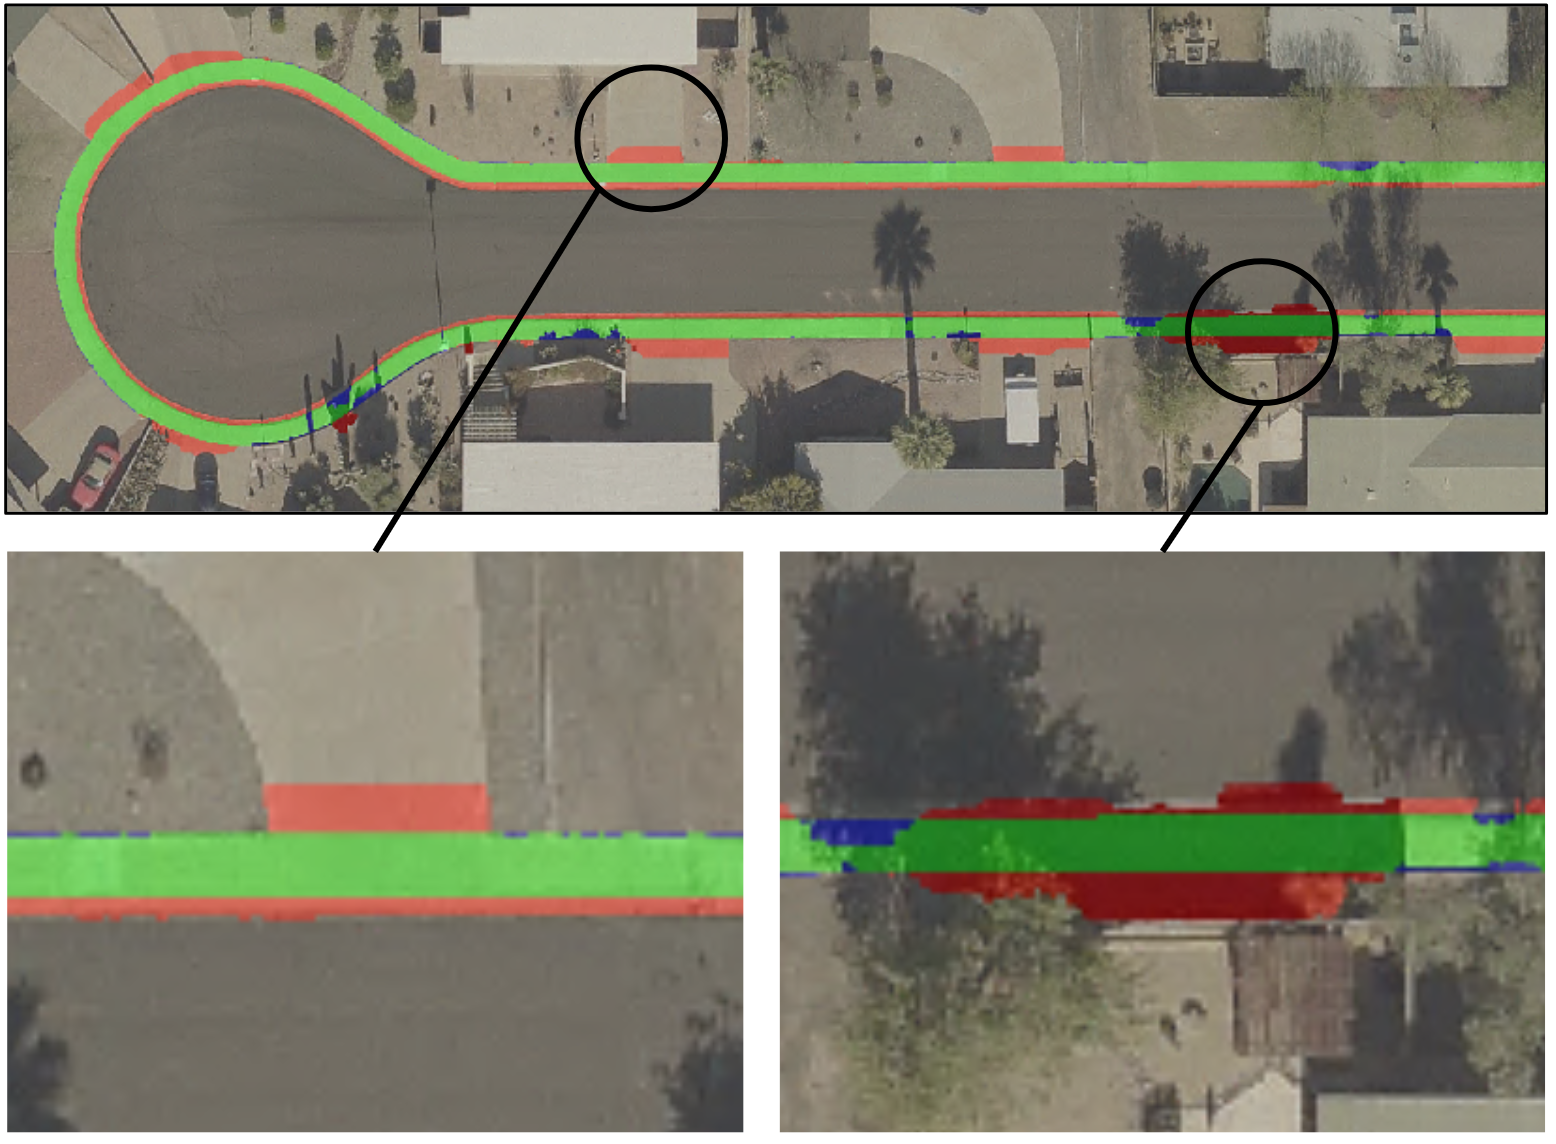
\includegraphics[width=\textwidth]{Figures/grabcut_sample.png} 
\caption[Example of \GrabCut{}]{
Details of our demonstration of the \GrabCut{} method. Row 2 indicates examples of errors, which are
\ac{FN} pixels recognized a non-sidewalk feature (shadow) and \ac{FP} pixels that have a similar
texture (driveway) as a part of sidewalk.}
\label{fig:grabcut}
\end{figure}

\GrabCut{} is a powerful image segmentation tool that combines both texture(color) and edge(contrast) information~\cite{Rother2004-ou}. 
It was designed to efficiently extract a foreground object from a complex background. 
As we illustrate in \figurename{} \ref{fig:Method_comparison} and \figurename{} \ref{fig:grabcut}, the overall
 performance on \GrabCut{} applied to a ribbon-like feature is fairly accurate, but it tends to to fail at identifying objects near the 
 sidewalk such as shadows, gutters or foliage. 
\GrabCut{} seems to identify the occluded regions as negative, we suspect that is because of the lack of width control.

\section {Super-pixels and Feature Extraction with SLIC}

\begin{figure}[H]
\centering
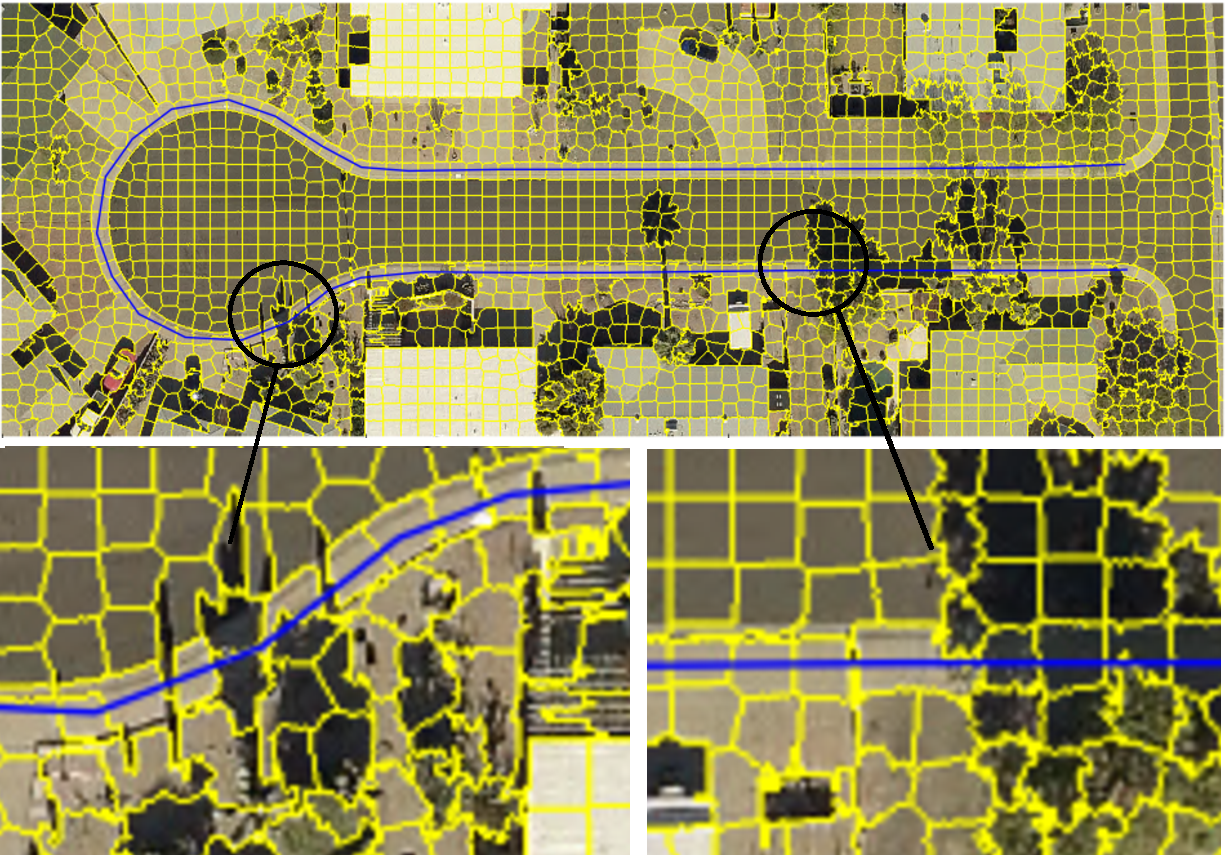
\includegraphics[width=\textwidth]{Figures/slic_sample1.pdf}
\caption[Example of Simple Linear Iterative Clustering]{
Detail of our demonstration of segmenting large image into irregularly shaped super-pixels with \ac{SLIC}.
Row 2 indicates examples of errors, with a non-sidewalk feature (shadow) recognized as a part of the sidewalk.}
\label{fig:slic}
\end{figure}

\acf{SLIC} is a method for identifying super-pixels, which segment a large image into different
irregularly shaped regions of homogeneous appearance or texture~\cite{Achanta:149300}. It finds
compact evenly distributed homogeneous regions of an image as a pre-processing step, so that image
segmentation can be accomplished by grouping super-pixels which snap to natural boundaries in an
image. Alternatively, super-pixels can initiate a region growing process~\cite{Borovec2017-fz}. As
shown in figure \ref{fig:slic}, \ac{SLIC} will identify a non-sidewalk feature as positive if there
is a shadow covering the sidewalk, which may lead to over mark the boundary (\acp{FP}). 
The results we show as \ac{SLIC} segmentation are superpixels that cross the original \ac{GIS} line strip.
When strong edges exist within the sidewalk (e.g. from shadows or occlusion) the \ac{SLIC} approach may
 fail to recognize part of the sidewalk (if the superpixel does not cross the line strip) or it may 
 detect objects that extend outside the sidewalk (if the superpixel crosses the line strip). 
Thus, finding a way to separate such a feature becomes
important. Trying to decrease the size or the width of each super-pixel is one of the ways to fix
this problem, but reducing the sizes of superpixels may result in poor recall of sidewalk pixels 
since each super-pixel is smaller than the width of the sidewalk.


\section{Active Contours}

\begin{figure}[H]
\centering
\includegraphics[width=\textwidth]{Figures/ac1.png}
\caption[Example of Active Contours]{
A detailed demonstration of the \ActiveContours{} method. 
Row 2 indicates examples of false positives, which recognized a non-sidewalk feature 
(shadow) and similar texture (driveway) as a part of sidewalk.}
\label{fig:ac}
\end{figure}

A very successful region growing process is snakes, or Active Contours, which starts with an approximate contour and evolves the boundary to optimize an energy function that favors likely contour shapes. 
%Compared with the other two segmentation tools, active contour may not be the best solution for identifying ribbon-like feature since it is not the best tool to separate blurred edges.
In general, it is biased towards segmenting compact regions with clear boundaries; but it has been used to segment blood vessels (which are ribbon-like features). 
Al-Diri~\cite{ActiveContou09} proposed using active contour to identify each edge of a vessel separately, while maintaining width consistency. 
The approach reported favorable results on blood vessel segmentation, but it is not ideal to apply on our problem, 
since their ribbon-like feature (vessels) does not requiring predict edges under obstacles,
 such as trees or cars that occlude the sidewalk.


Both \ac{SLIC} and active contours start from an initial shape to find precise boundaries by solving a \ac{CRF} problem. 
In addition, graph cuts are capable of global \ac{CRF} optimization in some situations, and iterative graph cut are used by the GrabCut algorithm to refine an initial segmentation~\cite{Rother2004-ou}. However in figure \ref{fig:Method_comparison} and figure \ref{fig:ac}, we show the segmentation results of these methods, and note that they struggle to constrain their results to ribbon-like shapes with smooth thickness and mid-line.
These color or boundary smoothness methods fail to capture an important quality of ribbon-like features, which is the thickness at one point depends not only its adjacent points but also its topologically distant points along the contour.

\section{Convolutional Neural Networks}

Another image segmentation approach that has seen extraordinary success is the use of Convolutional Neural Networks (CNNs) and transposed convolution~\cite{Badrinarayanan2017-il, Noh2015-ni, Shelhamer2017-rf, Ronneberger2015-sv}. 
Unlike the proposed approach, these have millions of tunable parameters and need significant pre-annotated data and offline training to build a model. 
In a recent exploration of learning to segment street networks from online maps, Kaiser et al.~\cite{Kaiser2017-np} built a fully convolutional network with 137 million parameters.
A similar approach with another deep architecture called U-net~\cite{Ronneberger2015-sv} was applied to the street network segmentation problem~\cite{Zhang2017-gi}.
These approaches claim to be robust to occlusion and ambiguous regions, but they benefit from a large amount of carefully annotated data that includes road width~\cite{Mnih2013-dp}. 
This type of pre-annotated data with aligned aerial imagery is much harder to obtain for walking paths. 
The proposed \ac{DPRST} approach has only a few tunable parameters with clear interpretations, so that they can be interactively set and used without offline training.


% \section{boss paper}